\section*{HOW TO}
\label{sec:usage}
This template is used for the student reports of the \coursename\ course. Remove this section by editing the \texttt{reportContent.tex} file \textbf{after} you have understood how to use this template.

\subsection*{Folder Structure}
\begin{lstlisting}[escapechar=!]
proceedings /
  |- reportContent /  <-- YOUR working folder
      |- images /     <-- Images are stored here
      |- sections /   <-- Additional sections / tex-files here
          |- _HOWTO_.tex    <-- *this* How To section
          |- introduction.tex
          |- report.bib
          |- lessons-learned.tex
          '- section2.tex
      '- reportContent.tex  <-- Change your section imports here
  |- !\rootDocument!  <-- DO NOT alter this file
  |- llncs.cls                            <-- NOR that
  |- proceedings.py                       <-- NOR that
  |- splncs03.bst                         <-- NOR that
  '- UniBas_Logo_EN_Schwarz_RGB_65.pdf    <-- NOR that
\end{lstlisting}
\ 

\subsection*{Setup}
Your report is compiled using the \texttt{\rootDocument} file. Therefore, we suggest that you set the file \texttt{\rootDocument} as the Master-/Root-Document that you can conveniently work on your report.
Please be aware that you have to compile the \texttt{\rootDocument} file in the following order:

\begin{enumerate}
    \item \verb|pdflatex| \rootDocument
    \item \verb|biber| \rootName
    \item \verb|pdflatex| \rootDocument
    \item \verb|pdflatex| \rootDocument
\end{enumerate}

For your convenience, you can compile this document by using the \texttt{proceedings.py} utility:

\begin{center}
    \verb|$> python proceedings.py -p|
\end{center}

And subsequently (especially before your submission) clean the auxiliary \LaTeX files:

\begin{center}
    \verb|$> python proceedings.py -z|
\end{center}


\subsection*{Images}
Images placed in the \texttt{images} sub-folder can be used directly in the \texttt{\textbackslash includegraphics} command -- see also \Cref{fig:rosette}. Also, sub-figures are possible: \Cref{fig:fly,fig:flies}.

Please \textsc{do~not} store your images elsewhere! 

Please use your group number (e.g., \textit{1}) in every image file name (e.g., \textit{g1-rosette.pdf} instead of \textit{rosette.pdf})!

\begin{figure}[tb]
\centering
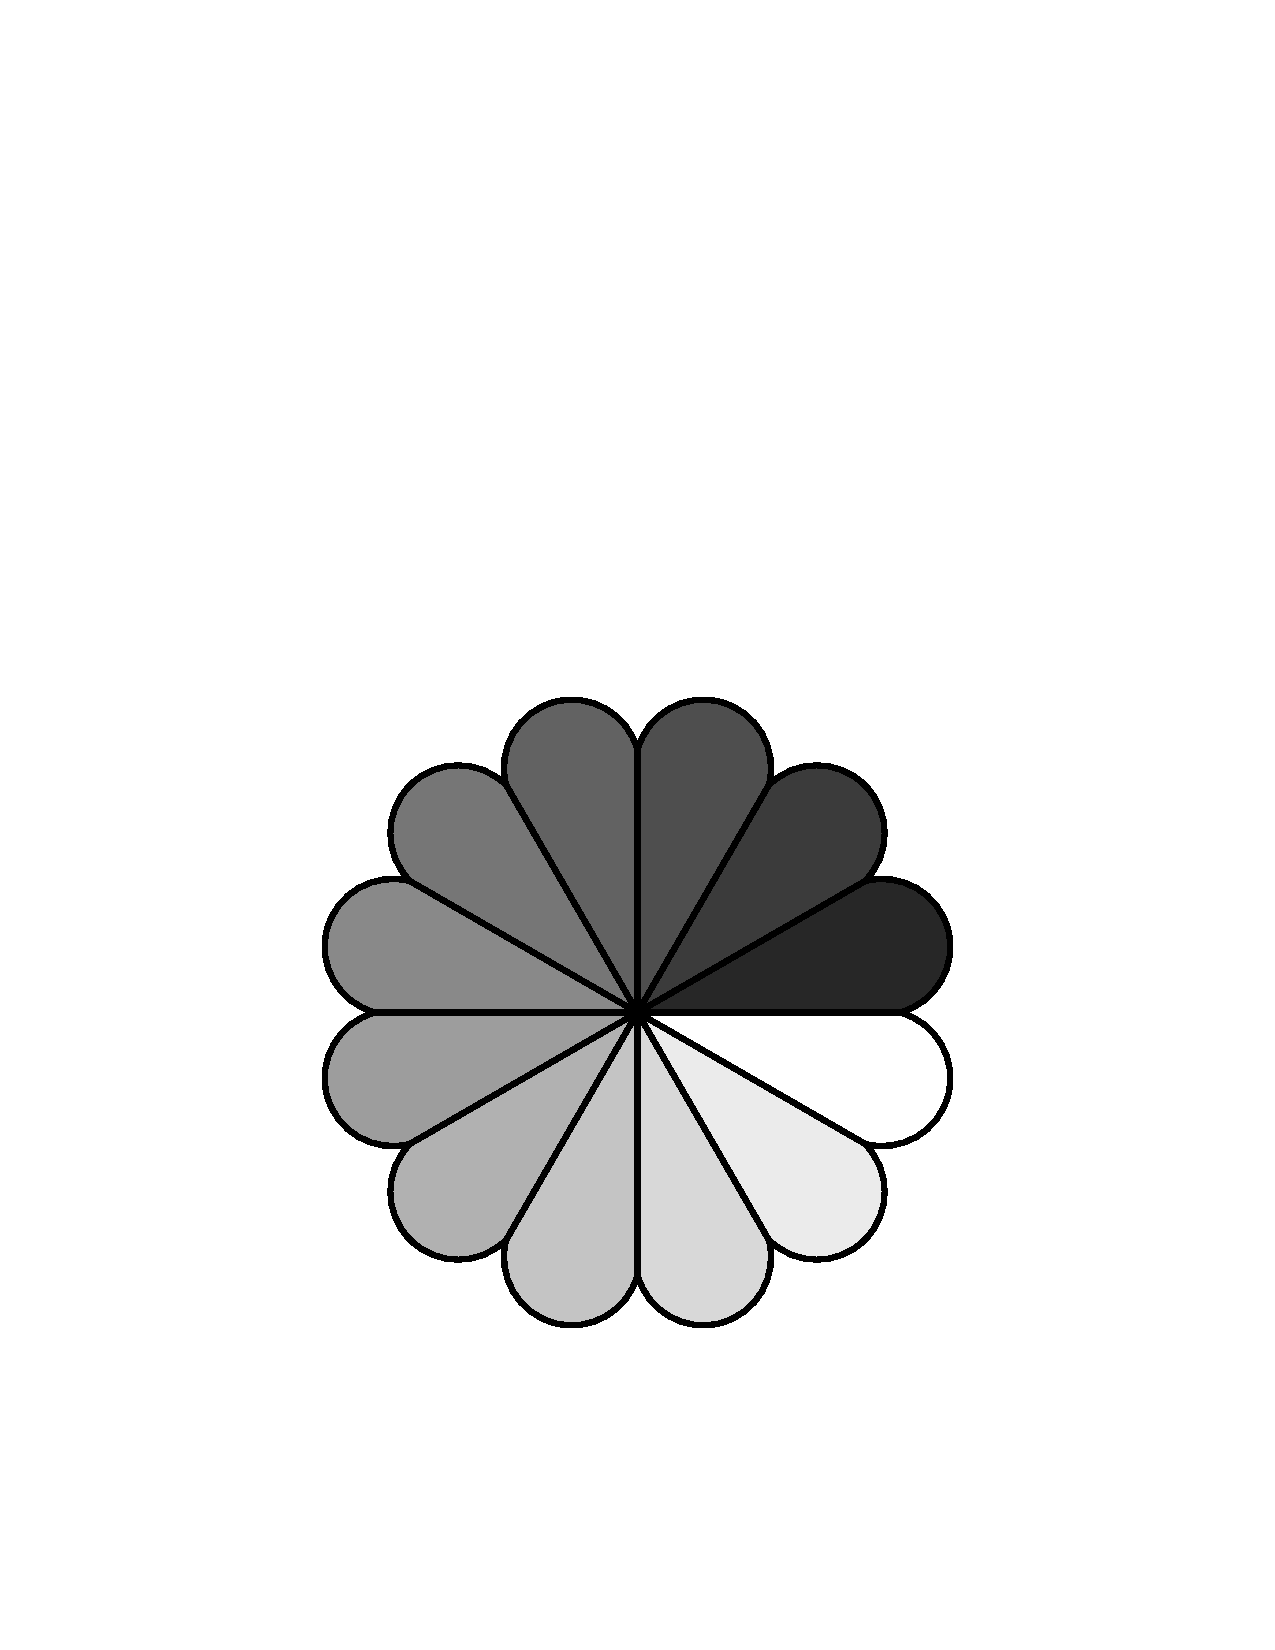
\includegraphics[width=0.45\textwidth]{g1-rosette}
\caption{Example figure stored in the \texttt{images} sub-folder and displayed with \texttt{\textbackslash includegraphics[width=0.45\textbackslash textwidth]\{g1-rosette\}}}
\label{fig:rosette}
\end{figure}

\begin{figure}[tb]
\centering
    %\subfloat[CAPTION]{BILDERCODE}\qquad
    \subfloat[A fly\label{fig:fly}]{
\includegraphics[width=0.4\textwidth]{g1-fly}}\qquad
    \subfloat[Flies\label{fig:flies}]{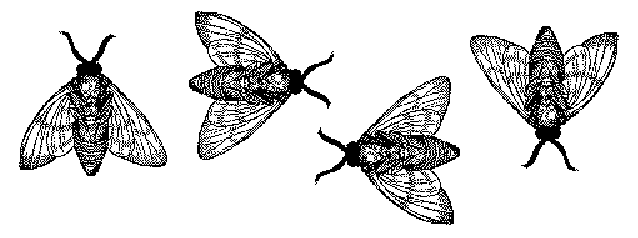
\includegraphics[width=0.45\textwidth]{g1-flies}}
\caption{Example figure stored in the \texttt{images} sub-folder}
\label{fig:example subfigure}
\end{figure}


\subsection*{Code}
To illustrate code use the \texttt{lstlisting} environment:
\begin{lstlisting}[language=Java]
public void foo( final int bar ) {
  System.out.println( bar );
}
\end{lstlisting}


\subsection*{Labels and References}
The proceedings template includes the package \textit{cleveref}, which enables pretty references. One such reference is the following one: \Cref{fig:example subfigure}, which was produced using the command \verb|\Cref{fig:example subfigure}|.
To use the full potential of such clever referencing, one have to set up labels, such as in the example before. The label command was \verb|\label{fig:example_subfigure}| (as seen in the source code in line 69).
Be aware that you have to prefix every single label you use with your group name, i.e. \verb|g1| to not clash with other group's labels.

\subsection*{Bibliography}
We use the \verb|biblatex| package with biber\footnote{\url{http://biblatex-biber.sourceforge.net/}} as backend, which most distributions already include.
Your references are stored in the \texttt{report.bib} file and used with the \texttt{\textbackslash cite} command. 
For example: \cite{kopka1995guide}. 
If the previous example shows \verb|kopka1995guide| - you need to re-run the compilation in the following order: pdflatex, biber, pdflatex, pdflatex.
In case you need some help with references in latex, there is an excellent cheatsheet\footnote{\url{http://tug.ctan.org/info/biblatex-cheatsheet/biblatex-cheatsheet.pdf}}.


\pagebreak